\documentclass[11pt,letterpaper]{article}
\usepackage{array}
\usepackage{fullpage}
\usepackage{graphicx}
\usepackage{parskip}
\usepackage{amsmath}
\usepackage[small]{caption}
\usepackage{graphpap}
\usepackage{logpap}
\usepackage{tabularx}
\usepackage{url}
\usepackage{hyperref}
\usepackage{enumitem}

\renewcommand{\thesection}{PART \arabic{section}: }

\newcounter{question}[section]
\newenvironment{question}[1][]{\refstepcounter{question}\par\medskip
   \textbf{\arabic{section}.\thequestion.} \rmfamily}{\medskip}

\usepackage{titlesec}
\titleformat{\section}{\clearpage\normalfont\bfseries}{\thesection}{0em}{}
\titlespacing{\section}{0pt}{0.5\baselineskip}{0pt}

\titleformat{\subsection}[runin]
{\normalfont\bfseries}{\thesubsection}{1em}{}

\titleformat{\subsubsection}{\normalfont\bfseries}{\thesubsubsection}{0em}{}
\titlespacing{\subsubsection}{0pt}{0.5\baselineskip}{0pt}

\newcounter{saveenumi}
\newcommand{\seti}{\setcounter{saveenumi}{\value{enumi}}}
\newcommand{\conti}{\setcounter{enumi}{\value{saveenumi}}}

\usepackage[dvipsnames]{xcolor}
\newcommand{\sol}[1]{{\color{NavyBlue} #1}}

\begin{document}
\setlength{\parindent}{0in}



\begin{flushright}
  PHYS S211: General Physics I\\
  Lab \#10: Sound waves\\
11/29/22 (due 12/9/22)
\end{flushright}

Name(s):\\

\subsubsection*{Topics:}
\begin{enumerate}
\setlength{\parskip}{3pt}
\item Sound recording
\item Basic properties of sound: frequency, pitch, and amplitude
\item Digital analysis of sound with Fast Fourier Transforms (FFTs)
\item Harmonics and doppler shifts
\end{enumerate}

\subsubsection*{Introduction:}
In this lab you will investigate sounds produced by tuning forks and by vibrations within tubes.  In order to quantitatively measure parameters of sound, you will use computer software designed to graphically display and measure sound. The broad goals of the lab are to learn
how to measure sounds and to identify characteristics that make sounds ``sound different''. Sounds surround us everyday. We have a natural understanding of loudness and other characteristics of sound, but most of us do not have a rigorous mathematical understanding (such as frequency or period).  

Graphical representations of sound are useful for comparing sounds and analyzing sources of sound.  While visual representations of sound may seem unusual, we are actually quite familiar with the idea---sheet music used by musicians is one example of a visual representation of sound:

\begin{figure}[h]
\begin{center}
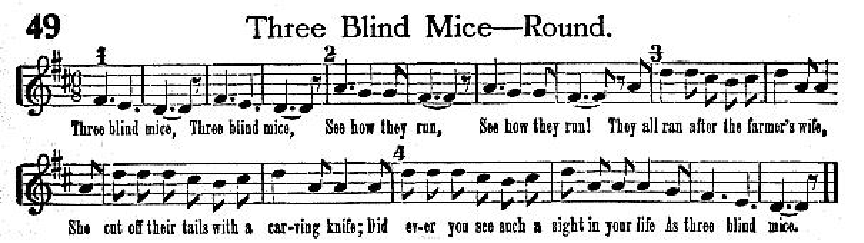
\includegraphics[width=0.8\textwidth]{./ThreeBlindMice}
\end{center}
\end{figure}

Sheet music is a prescriptive representation of a series of specific notes (frequencies), their duration, and their relationship in time.

\subsubsection*{What you should turn in:} 
You may submit a group report.
\begin{itemize}
\setlength{\parskip}{3pt}
\item Part 1: FFT graphs and calculated wavelengths of the two tuning forks in question 1 [3 pts]
\item Part 1: FFT and time series graphs of ``beats'' and calculated beat frequency from the graphs [4 pts]
\item Part 2: FFT graph demonstrating the Doppler shift and calculated speed with which you were moving the tuning fork [3 pts]
\item Part 3: Graph of $\log f$ vs $\log L$, curve fitting result, and response to questions [6 pts]
\item Part 4: Calculation of the frequency of the ``unknown'' tuning fork. [2 pts]
\end{itemize}

\subsubsection*{Equipment:}
\begin{itemize}
\setlength{\parskip}{3pt}
\item Labquest interfaces
\item Labquest microphones
\item tuning forks
\item metal and plastic pipes
\item resonance tubes
\end{itemize}

\section{SOUND FREQUENCY AND AMPLITUDE}
Using Logger Pro software, you will measure the frequency and amplitude of sound waves produced by tuning forks (which emit sound at specific frequencies). Before making measurements, first spend some time playing with the tuning forks and software to become familiar with the sound data acquistion.

LoggerPro has two sampling modes that you should experiment with---triggered and untriggered sampling. The triggering mode depends on the sound exceeding a threshold and may be difficult to use in some cases, whereas the untriggered sampling can be difficult to use if you are trying to isolate a specific sound. You will want to make use of both modes throughout this lab. Another data acquisition option is the sample rate and the number of samples to acquire. You should check your acquisition software settings to see the time between samples (making measurements from the amplitude versus time plots). Try using the Fast Fourier Transform (FFT) plot by ``adding an additional plot''. The Fast Fourier Transform is essentially a mathematical tool for decomposing a waveform into sine and cosine waves. A single FFT of a waveform shows what frequencies are present in the signal, as shown in the example below.

\begin{figure}[h]
\begin{center}
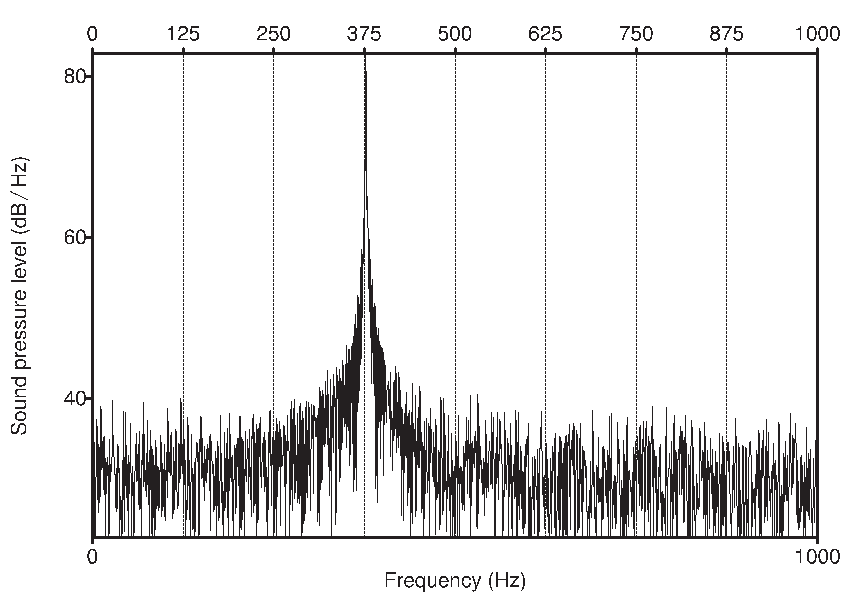
\includegraphics[]{./fft_zoom}
\end{center}
\end{figure}

Now that you are familiar with the software, do the following exercises:
\begin{enumerate}
\item Plot the FFT for two different tuning forks, and submit the results. Indicate the frequency of the tuning fork as measured by LoggerPro. For this example you will likely want to use the triggered sampling mode. In addition, calculate the wavelength of the sound waves produced by the tuning forks. The speed of a wave is related to the wavelength $\lambda$ and frequency $f$ by
\begin{equation*}
v=\lambda f.
\end{equation*}
For sound waves traveling through air at 20$^\circ$C and 1 atm, $v=343$~m/s.
\item Now switch to untriggered sampling and set the duration to 1~s. Find two tuning forks with similar frequencies (within 5--10~Hz of each other). Get them both ringing, hold them close to the microphone, and then hit collect. This should produce what is referred to as ``beats'', which are \textit{oscillations in sound intensity} that occur due to constructive and destructive interference of the sound waves. Submit two graphs: one that shows the pulses in intensity over time, and one FFT graph that shows the frequencies of the tuning forks. From the time series graph, estimate the beat frequency (i.e., measure the period between subsequent peaks in intensity and take the reciprocal).

\end{enumerate}

\section{DOPPLER SHIFT}
When a wave source is traveling toward or away from you, the frequency that you hear is different than the frequency of sound that is being emitted. This is referred to as the Doppler shift, which is responsible for the characteristic change in pitch that you hear when a police car passes you (or a race car goes around a track).

The frequency that you observe, $f_o$, depends on the speed with which the source is moving:
\begin{equation}
f_o=\left(\frac{v}{v\mp{v_s}}\right)f,
\end{equation}
where $v=343$~m/s is the speed of sound, $v_s$ is the speed at which the source is moving, $f$ is the frequency that is actually being emitted, and the denominator has a negative (positive) sign if the source is moving toward (away) from the receiver. 

Use a tuning fork of about 250~Hz. Use the untriggered mode and a duration of 1~s. First, get the tuning fork ringing, hold it steady next to the microphone, and hit record. When you plot the FFT you should observe a single peak around 250~Hz. Now, repeat, but this time quickly flick your wrist back and forth so that the tuning fork is rapily moving toward and away from the microphone. This may take a few tries, but eventually you should be able to be produce a FFT graph that  has multiple peaks around 250~Hz. There should be one peak with a frequency that matches the natural frequency of the tuning fork, as well as one (or more) peaks with slightly higher and slightly lower frequencies that correspond to time periods during which the tuning fork was moving toward/away from the microphone. The FFT graph plots frequencies that were present at any time during the 1~s interval, so these frequencies were not present at the same time. Submit this FFT graph to demonstrate that you were able to produce a frequency shift, and then use the observed frequencies to estimate the speed maximum speed of the tuning fork as you flicked it back and forth. If your FFT graph shows multiple peaks, use the peaks immediately adjacent to the natural frequency of the tuning fork.


\section{FREQUENCIES PRODUCED BY TUBES}
Air in a tube vibrates at specific frequencies that depend on the length of the tube and whether the ends of the tube are open or closed. The lowest frequency vibration of a tube is referred to as the fundamental frequency. However, tubes also produce sounds with frequencies that are integer multiples of the fundamental frequency. These higher frequencies are referred to as harmonics. For tubes that are closed on one end, only odd harmonics will be produced.

For this exercise, you should determine the relationship between the fundamental frequency and the length of open-closed tubes (one end is open and the other end is closed). Use four different length tubes. Set LoggerPro to the triggered mode, and point the end of the tube at the microphone. Hit the end of the tube that is away from the microphone with an open palm, and keep your hand on the end of the tube after making contact. Produce an FFT graph and determine the lowest frequency that was produced by the tube. For short tubes, it should be pretty easy to identify the lowest frequency but the harmonics might be difficult to spot. For the long tubes, you will see numerous harmonics but might have trouble determining the fundamental frequency. If this is the case, you can look at the difference between successive harmonics, which will equal two times the fundamental frequency (since only odd harmonics are produced).

If you plot frequency (y-axis) vs. tube length (x-axis), you will see that the relationship is not linear. Instead, plot $\log f$ vs $\log L$, which should plot as a straight line. Find the slope and y-intercept of this line. Submit this graph and the results of the curve fitting. Translate the slope and y-intercept into a relationship of the form
$$f = aL^b$$
(We've done this in lab several times this semester.) The exponent $b$ should be very close to an integer value. Assuming that it should equal that integer value, what units must the constant $a$ have? What might this tell you about how the frequency of an open-closed tube depends on other properties of sound waves?



\section{RESONANCE}
In the previous lab you learned that resonance occurs when a system is being forced at a frequency that corresponds to the natural frequency of the system. This also applies to vibrations in a tube. If you hit a tuning fork and hold it close to the mouth of a tube, it will try to force the tube to vibrate at that frequency. If the tuning fork has the same frequency as the fundamental frequency or one of the harmonic frequencies of the tube, then resonance will occur and the sound will become relatively large.

You can use this idea, along with your results from the previous exercise, to determine the frequency of an ``unknown'' tuning fork (I have covered the marking with tape). A resonance tube allows you to adjust the tube length by raising or lowering the water level in the tube. Hit the tuning fork, hold it over the water-filled tube, and let the water drain. As the water drains the tube length is increasing. At some point the natural frequency of the tube will be the same as frequency of the tuning fork and resonance will occur. Note the water height at which this occurs, and measure the tube length. From there you should be able to calculate the frequency of the tuning fork---keeping in mind that you may be observing a harmonic of the fundamental frequency. You should test to see whether you can get resonance to occur for different tube lengths.

Report your observed frequency.

\end{document}
